\begin{figure}[h!]
\centering
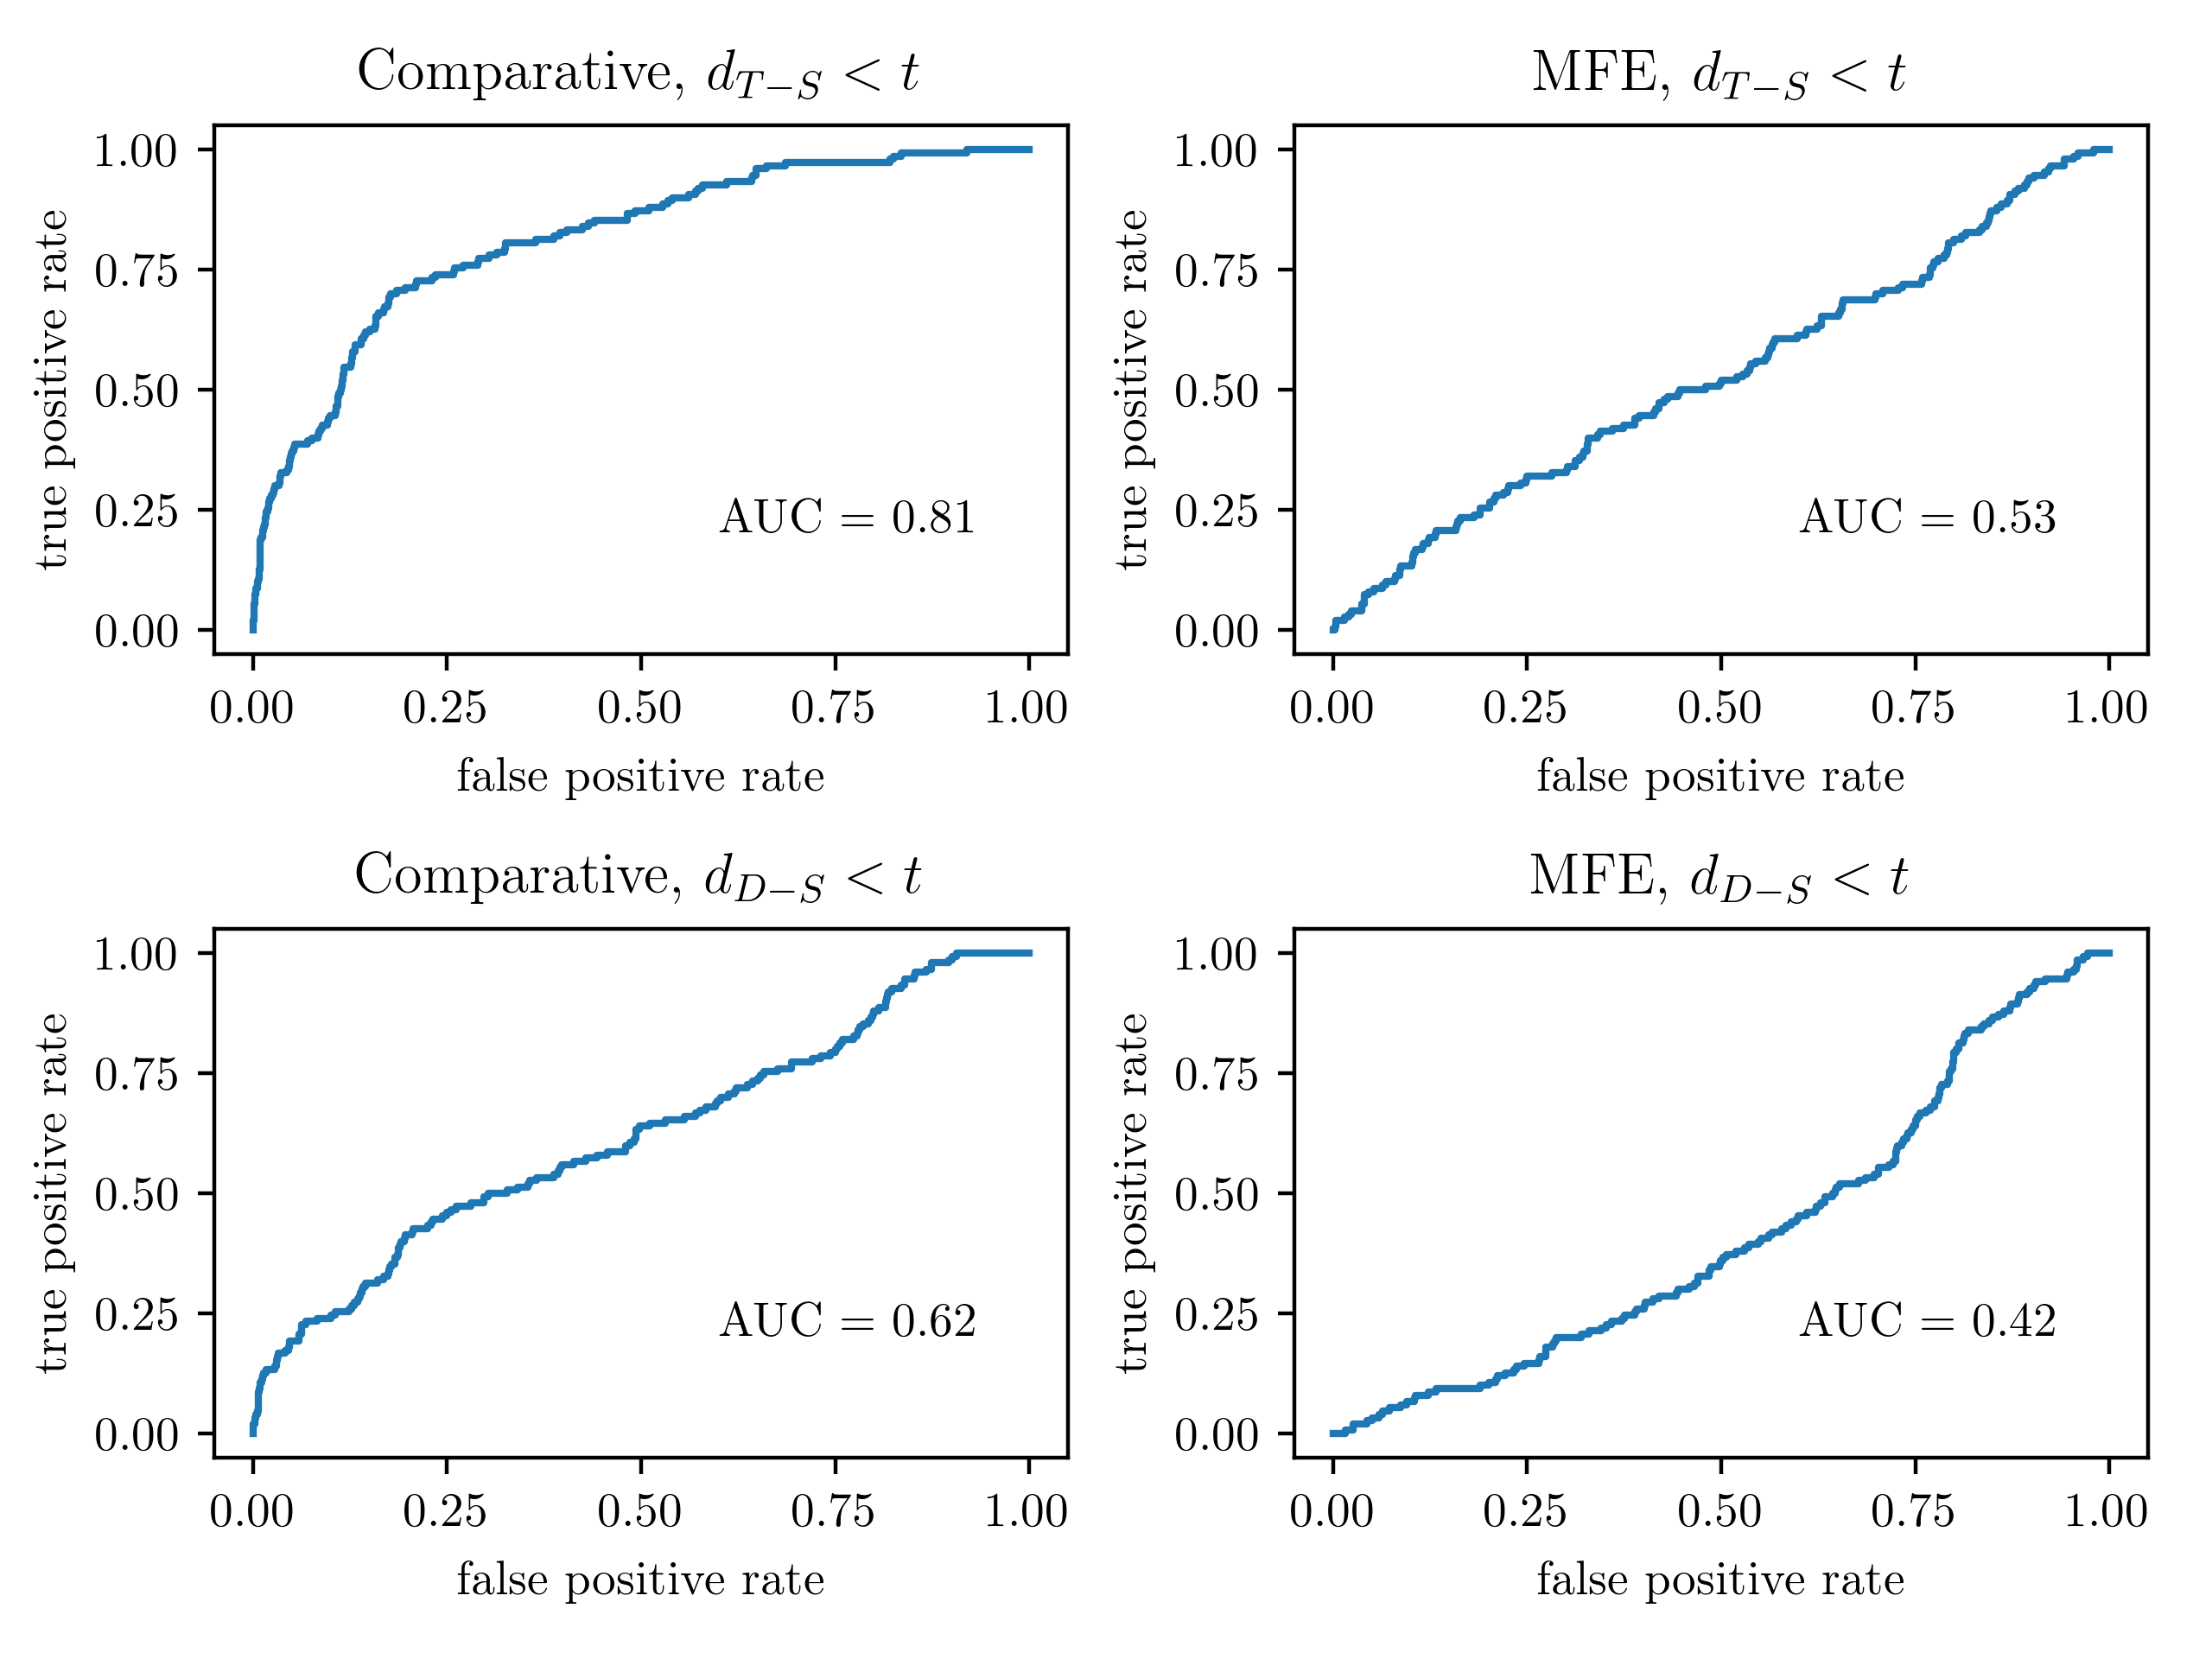
\includegraphics[width=\textwidth]{bound_unbound.png}
\vglue 0.5cm

\caption{{\bf Bound or Unbound?} ROC performance of classifiers based on thresholding T-S
and D-S ambiguity indexes. Small values are taken as evidence for molecules that are active as
single entities (unbound), as opposed to parts of ribonucleoproteins (bound). Classifiers in the
left two panels use comparative secondary structures to compute ambiguity indexes; those on the
right use (approximate) minimum free energies. In each of the four experiments, a conditional
p-value was also calculated, based only on the signs of the indexes and the null hypothesis that
positive indexes are distributed randomly among molecules of all types as opposed to the alternative
that positive indexes are more typically found among families of bound RNA. Under the null hypothesis,
the test statistic is hypergeometric---see Eq \ref{eqn:null}. {\em Upper Left:} $p= 1.2 \times 10^{-34} $;
{\em Lower Left:} $p=7.3 \times 10^{-8}$; {\em Upper Right:} $p=0.02$;  {\em Lower Right:} $p=0.92$.
In considering these extreme p-values, it is perhaps worth re-emphasizing the points made about the
interpretation of p-values in the paragraph following Eq \ref{eqn:null}. (These ROC curves and
those in Figure \ref{fig:CompVSMFE} were lightly smoothed by the method known as
``Locally Weighted Scatterplot Smoothing,'' e.g. with the python command Y=lowess(Y, X, 0.1, return\_sorted=False)
coming from \textit{statsmodels.nonparametric.smoothers\_lowess}.)
}
\label{fig:UnboundVSBound}
\end{figure}
